%!TeX root=../main.tex
\قسمت{مقدمه}
ایستگاه هواشناسی، مرکزی مجهز به تجهیزات و ابزارهایی برای اندازه‌گیری‌های جوی است که به ارائه اطلاعات برای پیش‌بینی و مطالعه آب‌وهوا می‌پردازد. اندازه‌گیری انجام‌شده معمولاً شامل دما، فشار هوا، رطوبت، سرعت باد، جهت باد و مقدار بارش است. مشاهدات دستی حداقل یک بار در روز انجام می‌شود، درحالی‌که اندازه‌گیری خودکار حداقل یک بار در ساعت انجام می‌پذیرد.

ایستگاه‌های هواشناسی معمولی مجهز به ابزارهای زیر هستند \مرجع{wikipedia:Weather_station}:

\شروع{فقرات}
\فقره
رطوبت‌سنج برای اندازه‌گیری رطوبت
\فقره
فشارسنج برای اندازه‌گیری فشار جو
\فقره 
دماسنج برای اندازه‌گیری دمای هوا
\فقره
پیرانومتر برای اندازه‌گیری تشعشعات خورشیدی
\فقره
باران‌سنج برای اندازه‌گیری میزان بارش باران در طی یک دوره زمانی مشخص
\فقره
تجهیزاتی نظیر بادسنج، پرچم باد یا جوراب باد برای اندازه‌گیری سرعت و جهت باد
\پایان{فقرات}

ایستگاه‌های پیشرفته‌تر همچنین ممکن است شاخص فرابنفش، رطوبت برگ، رطوبت خاک، دمای خاک، دمای آب در حوضچه‌ها، دریاچه‌ها، نهرها یا رودخانه‌ها و گاهی داده‌های دیگر را اندازه‌گیری کنند. به‌جز دستگاه‌هایی که نیازمند تماس مستقیم با عناصر مورداندازه‌گیری هستند (نظیر بادسنج)، دیگر سنسورها و دستگاه‌ها باید در محفظه‌ای به‌دوراز تابش مستقیم خورشید و وزش باد قرار بگیرند.

ایستگاه‌های هواشناسی سینوپتیک (\متن‌لاتین{Synoptic}) 24 ساعته به‌صورت خودکار هر سه ساعت به سه ساعت پارامترهای جوی را پس از اندازه‌گیری و جمع‌آوری از طریق شبکه‌های مخابراتی منتقل می‌کنند. به‌طور مشابه ایستگاه‌هایی با نام متار (\متن‌لاتین{Metar}) این کار را هر  یک ساعت انجام می‌دهند. وظیفه این ایستگاه‌ها جمع‌آوری اطلاعات جوی از محدوده‌هایی وسیع و مخابره به ایستگاه‌های اصلی به‌منظور اطلاع از وضعیت حال و گذشته و پیش‌بینی شرایط آب و هوایی مناطق در آینده است. 

هدف این پروژه پیاده‌سازی نوعی ایستگاه هواشناسی سینوپتیک است که با تجهیزات ارزان و کم‌مصرف دیجیتالی پارامترهای جوی لازم را جمع‌آوری و به‌صورت بی‌سیم به ایستگاهی جهت ثبت و نمایش مخابره می‌کند. در این پروژه از میکروکنترلر (\متن‌لاتین{Microcontroller}) \متن‌لاتین{ARM} سری \متن‌لاتین{STM32F10X} به‌عنوان هسته اصلی پردازش در هر دو سمت سنسور و ایستگاه و از ماژول لورا (\متن‌لاتین{LoRa}) با چیپ \متن‌لاتین{SX1278} به‌منظور برقراری ارتباط بی‌سیم استفاده شده ‌است.

\قسمت{اجزای سیستم}

این سیستم به دو دستگاه اصلی تقسیم می‌شود، یک دستگاه جهت جمع‌آوری اطلاعات جوی برروی یک میله در ارتفاع 10 متری سطح زمین قرار می‌گیرد و اطلاعات جوی نظیر دما، رطوبت، فشار، شدت نور، سرعت و جهت باد را از سنسورهای مربوطه جمع‌آوری کرده و به‌صورت بی‌سیم به دستگاه دیگر، که در ایستگاه اصلی قرار دارد، مخابره می‌کند؛ سپس اطلاعات دریافت شده در سمت دستگاه دوم جهت ثبت و ذخیره به رایانه منتقل می‌شود. در اینجا به دستگاه اول که وظیفه جمع‌آوری اطلاعات جوی را دارد سنسور و دستگاه دوم که وظیفه دریافت اطلاعات مخابره شده و انتقال به رایانه را دارد ایستگاه می‌گوییم. بلوک دیاگرام کلی این سیستم و نحوه ارتباط بخش‌های مختلف با یکدیگر در شکل \رجوع{fig:systemDesign} آمده است.

\begin{figure}[!h]
	\centering
	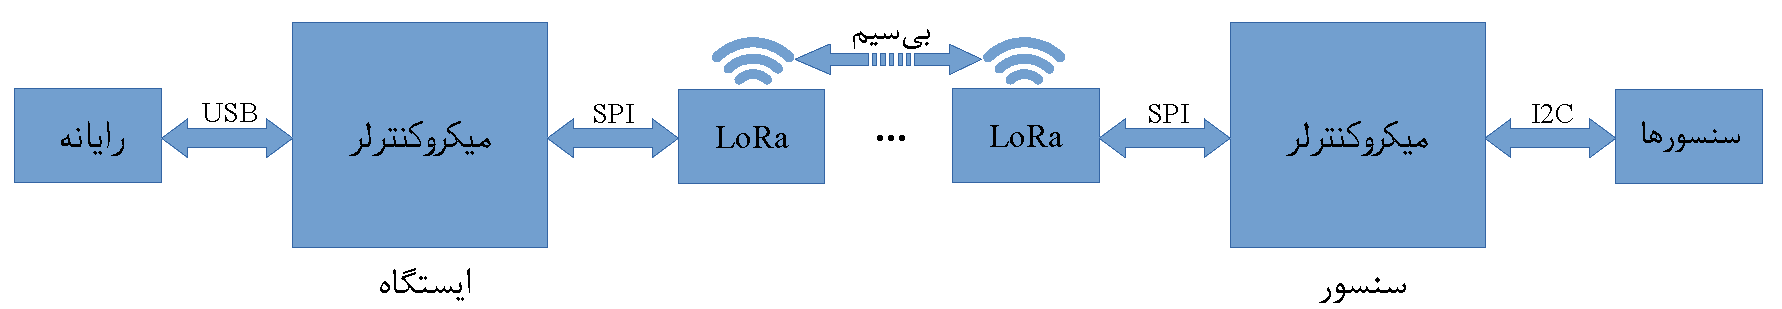
\includegraphics[width=\linewidth]{Assets/system design.pdf}
	\caption{بلوک دیاگرام اجزای سیستم و نحوه ارتباط اجزای مختلف با یکدیگر.}
	\label{fig:systemDesign}
\end{figure}

\زیرقسمت{میکروکنترلر}

هسته اصلی پردازش در هر دو سمت ایستگاه و سنسور میکروکنترلر \متن‌لاتین{STM32f103CBT6} انتخاب شده است که با توجه به موجود بودن در بازار ایران و دارا بودن 2 عدد \متن‌لاتین{I\بالانویس‌متنی{2}C}\پانویس{Inter-Integrated Circuit}، 2 عدد \متن‌لاتین{SPI}\پانویس{Serial Peripheral Interface}، اینترفیس\پانویس{Interface} \متن‌لاتین{USB}\پانویس{Universal Serial Bus} و 3 عدد تایمر 16 بیتی نیاز به حداقل 1 عدد \متن‌لاتین{I\بالانویس‌متنی{2}C} (در سمت سنسور)، 1 عدد \متن‌لاتین{SPI} (در هر دو سمت)، اینترفیس \متن‌لاتین{USB} (در سمت ایستگاه)  و 1 عدد تایمر (در سمت سنسور) را برآورده می‌کند. همچنین حالت \متن‌لاتین{Sleep} و واحد \متن‌لاتین{RTC} موجود در این میکروکنترلرها به کاهش مصرف انرژی در وقفه‌های سه ساعته کمک می‌کند؛ به‌طوری‌که استفاده از سیستم باتری و پنل خورشیدی را ممکن می‌سازد.

\زیرقسمت{ارتباط بی‌سیم}

به‌طورکلی در این سیستم مصرف پایین انرژی به دلیل استفاده از سیستم باطری و پنل خورشیدی بسیار اهمیت دارد. استفاده از شبکه تلفن همراه\پانویس{The Global System for Mobile Communications (GSM)} به‌عنوان راه‌حلی ابتدایی برای ارتباط بی‌سیم، علاوه بر نداشتن صرفه اقتصادی مصرف انرژی زیادی را به سیستم تحمیل می‌کند. همچنین تضمینی برای وجود پوشش شبکه تلفن همراه در مناطقی که قرار است داده‌های جوی از آن جمع‌آوری شود وجود ندارد. ازاین‌رو بهترین رویکرد استفاده از گیرنده و فرستنده‌های رادیویی در باندهای فرکانسی بدون نیاز به مجوز (\متن‌لاتین{ISM}) است. از میان گزینه‌های موجود ماژول‌های لورا\پانویس{LoRa (Long Range)} به لطف مدولاسیون \متن‌لاتین{CSS\پانویس{Chirp Spread Spectrum}} که از آن بهره می‌برند دارای مصرف توان پایین، ناحیه پوشش وصیع و نفوذپذیری مناسبی هستند که کاملاً با نیازهای ما سازگار است.

ماژول \متن‌لاتین{LoRa Ra-02} با تراشه \متن‌لاتین{Sx1278} دارای رنج فرکانسی 410 تا 525 مگاهرتز، و توان انتقالی ماکسیموم 18\متن‌لاتین{dBm} است و از مدولاسیون‌های \متن‌لاتین{LoRa}، \متن‌لاتین{FSK}\پانویس{Frequency Shift Keying} و \متن‌لاتین{OOK}\پانویس{On Off Keying} پشتیبانی می‌کند. برای ارتباط بی‌سیم در این پروژه از این ماژول استفاده‌شده است. 

\زیرقسمت{سنسورها} 

به‌منظور استخراج داده‌های جوی نظیر دمای هوا، رطوبت، فشار، شدت نور و... از سنسورهای دیجیتال استفاده می‌شود. این سنسورها علاوه بر کم‌مصرف بودن دارای دقت بالا و تأخیر پایینی در اندازه‌گیری پارامترهای موردنظر هستند. با دارا بودن این ویژگی‌ها این سنسورها کاملاً با سیستم تغذیه باتری و سلول خورشیدی سازگار هستند.

\زیرزیرقسمت{فشارسنج}

تغییرات فشار جوی یکی از عناصر مهم در پیش‌بینی وضعیت آب‌وهوا است. فشارسنج‌های جیوه‌ای از اواخر قرن 16 جهت پیش‌بینی وضعیت آب‌وهوا مورداستفاده قرار می‌گرفت. به‌طورکلی تغییر فشار هوا رو به بالا نشان‌دهنده آسمان آفتابی، گرم و صاف و تغییر فشار هوا رو به پایین نشان‌دهنده بارش باران، طوفان و آسمانی مملو از ابرهای باران‌زا است. علاوه بر این فشار هوا یکی از عوامل مؤثر در سنجش سرعت باد نیز به شمار می‌آید. 

سنسور استفاده‌شده برای این منظور ماژول سنسور \متن‌لاتین{BMP180} است که با مصرف جریان تنها در حد چند میکرو آمپر دقتی معادل با 0٫3 هکتوپاسکال\پانویس{Hectopascal (hPa)} دارد و توانایی اندازه‌گیری فشار هوا در بازه 300 تا 1100 هکتوپاسکال را دارا است. نحوه ارتباط با این ماژول از طریق رابط \متن‌لاتین{I\بالانویس‌متنی{2}C} است. 

\زیرزیرقسمت{شدت نور}

شدت نور خورشید یکی از پارامترهای اصلی سنجش وضعیت آب‌وهوا است. از این سنسور جهت نشخیص ابری یا آفتابی بودن هوا می‌توان استفاده کرد. همچنین به دلیل اهمیت موضوع سلامت پوست، معمولاً در کنار این سنسور از سنسور سنجش شدت \متن‌لاتین{UV} به‌منظور اطلاع‌رسانی شدت \متن‌لاتین{UV} نیز استفاده می‌شود. 

جهت سنجش شدت نور از ماژول سنسور \متن‌لاتین{MAX44009} استفاده‌شده است که با 0٫65 میکرو آمپر مصرف جریان در هنگام کارکرد شدت نور در بازه‌ی 0٫045 لوکس تا 188 هزار لوکس را اندازه‌گیری می‌کند. همچنین اینترفیس ارتباطی این ماژول رابط سریالی \متن‌لاتین{I\بالانویس‌متنی{2}C} می‌باشد.

\زیرزیرقسمت{قطب‌نما}

ازآنجایی‌که این دستگاه در سمت سنسور معمولاً در ارتفاع 10 متری زمین روی یک میله نصب می‌شود، قرار دادن دستگاه در جهت جغرافیایی خاص، به جهت سنجش جهت باد، ممکن است دشوار باشد (یا حتی خیلی دقیق نباشد). باوجود سنسور قطب‌نما در این دستگاه (برخلاف برخی دستگاه‌های مشابه) دیگر نیازی به نصب دستگاه در جهت جغرافیایی خاص نخواهد بود.

سنسور استفاده‌شده برای این منظور سنسور \متن‌لاتین{QMC5883L} است. که با ماکسیموم 100 میکرو آمپر جریان مصرفی می‌توان به‌دقت یک تا دو درجه در جهت‌یابی رسید. همچنین طریقه ارتباط این سنسور با میکروکنترلر از طریق رابط \متن‌لاتین{I\بالانویس‌متنی{2}C} است.

\زیرزیرقسمت{دما و رطوبت هوا}

درکتار وضعیت آسمان (ابری، آفتابی، بارانی و... بودن) معمولاً به‌طور مستقیم پارامتر دمای هوا نیز در اطلاع‌رسانی وضعیت و پیش‌بینی آب‌وهوا نقش ایفا می‌کند. در کنار این موارد رطوبت هوا نیز، علاوه بر نقشی که در پیش‌بینی دارد، معمولاً به‌طور مستقیم به سمع و نظر مخاطبین می‌رسد. علاوه این رطوبت نسبی هوا در کنار دمای هوا نقش مهمی در رسیدن به آسایش حرارتی در بدن انسان (و موجودات) دارد. به‌طوری کلی در دمای هوای بالاتر به رطوبت نسبی کمتری نسبت به دمای هوای پایین‌تر برای رسیدن به سطح آسایش  حرارتی نیاز است \مرجع{Schiavon2013}. 

ماژول سنسور \متن‌لاتین{AHT10} دما و رطوبت نسبی هوا را با دقت 0٫01 درجه سلسیوس\پانویس{Celsius} و 0٫024 درصد با تنها 3٫3 میکرو وات مصرف توان اندازه‌گیری می‌کند. همچنین این ماژول در رطوبت 0 تا 100 درصد و دمای  40- تا 100 درجه‌ی سلسیوس قابل‌استفاده است. خروجی این ماژول نیز سیگنال دیجیتال ارتباطی \متن‌لاتین{I\بالانویس‌متنی{2}C} است. 

\زیرزیرقسمت{شدت و جهت باد}

روش‌های مختلفی برای سنجش شدت باد وجود دارد، عمدتاً در این کاربرد دو روش سنجش مکانیکی و آلتراسونیک \پانویس{Ultrasonic} مورداستفاده قرار می‌گیرد. در سنجش شدت و جهت باد در روش مکانیکی از دو ابزار که به‌صورت مستقل کار می‌کنند (در برخی موارد این دو ابزار در قالب یک دستگاه در کنار هم قرار می‌گیرند) استفاده می‌شود، به طوری که یک ابزار برای سنجش شدت و ابزاری دیگر برای تعیین جهت، مورداستفاده قرار می‌گیرد. هر دو دستگاه دارای قطعات متحرک‌اند و یکی با داشتن پره‌هایی شبیه به دم هلی‌کوپتر با وزرش باد در جهت وزش قرار می‌گیرد و دیگری دارای پره‌هایی است که با وزش باد پره‌ها همانند پره‌های توربین به حرکت درمی‌آید که با توجه به‌سرعت چرخش پره‌ها سرعت باد قابل‌اندازه‌گیری است. در اندازه‌گیری‌های این دستگاه‌ها محدودیت‌هایی وجود دارد و اغلب این نوع ابزارها در وزش باد ملایم عملکرد صحیحی از خود نشان نمی‌دهند. همچنین در اندازه‌گیری زاویه وزش ممکن‌ است محدود به اندازه گیری زوایای خاصی باشند. 

در روش اندازه‌گیری شدت و جهت باد با آلتراسونیک اندازه‌گیری‌ها می‌تواند در قالب تنها یک دستگاه، بدون قطعات متحرک و با دقتی بالاتر انجام پذیرد. در این روش 2 فرستنده و گیرنده آلتراسونیک همان‌طور که در شکل \رجوع{fig:oneAxisUltrasonic} نشان داده‌شده است روبروی یکدیگر در فاصله مشخص $d$ قرار داده می‌شوند.

\begin{figure}[!h]
	\centering
	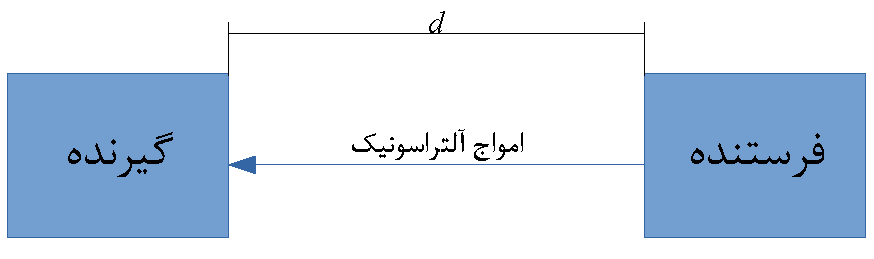
\includegraphics[width=0.6\linewidth]{Assets/ultrasonic one axis.pdf}
	\caption{نحوه قرارگیری فرستنده و گیرنده آلتراسونیک.}
	\label{fig:oneAxisUltrasonic}
\end{figure}

فرستنده امواج صوتی با فرکانس 40 کیلوهرتز (که برای گوش انسان قابل شنیدن نیست) تولید می‌کند. فاصله زمانی بین ارسال امواج صوتی از فرستنده و دریافت این امواج در گیرنده اندازه‌گیری می‌شود. با توجه به رابطه \رجوع{eq:speed}، سرعت $v$ با داشتن فاصله $d$ و زمان تأخیر بین ارسال موج صوتی در فرستنده و دریافت آن در گیرنده  $t$، قابل‌اندازه‌گیری است.

\begin{equation}\label{eq:speed}
	v = \frac{d}{t}
\end{equation}

سرعت $v$ به‌دست آمده از این رابطه مطابق رابطه \رجوع{eq:expandSpeed} متشکل از سرعت صوت $v_s$ و سرعت باد $v_{wx}$  است \مرجع{7988049}.

\begin{equation}\label{eq:expandSpeed}
	v = v_s + v_{wx}
\end{equation}

درصورتی‌که وزش باد در جهت موافق حرکت امواج صوتی باشد زمان تأخیر در دریافت امواج نسبت به حالی که باد نوزد کمتر شده و درنتیجه سرعت $v$ نسبت به حالتی که باد نوزد افزایش می‌یابد (یعنی علامت $v_{wx}$ مثبت بوده و $v = v_s+v_{wx}$). درصورتی‌که وزش باد در خلاف جهت حرکت امواج صوتی باشد زمان تأخیر در دریافت امواج نسبت به حالتی که باد نوزد بیشتر شده و درنتیجه سرعت $v$ کاهش می‌یابد (یعنی علامت $v_{wx}$ منفی بوده و $v = v_s-v_{wx}$). با داشتن سرعت صوت $v_s$، فاصله $d$ و محاسبه زمان $t$ می‌توان با توجه به معادلات \رجوع{eq:speed} و \رجوع{eq:expandSpeed} سرعت باد $v_{wx}$ و جهت باد (علامت سرعت $v_{wx}$) روی یک محور مطابق رابطه \رجوع{eq:speedWindX} به‌دست آورد. 

\begin{equation}\label{eq:speedWindX}
	v_{wx} = \frac{d}{t} - v_s
\end{equation}

به‌منظور سنجش شدت و جهت باد در دو بعد می‌توان دو فرستنده و گیرنده دیگر بر روی محوری عمود بر محور متصل‌کننده فرستنده و گیرنده فعلی قرارداد و با محاسبه دو بردار سرعت، بردار سرعت برآیند را به‌دست آورد.

\begin{figure}[!h]
	\begin{subfigure}[b]{0.5\textwidth}
		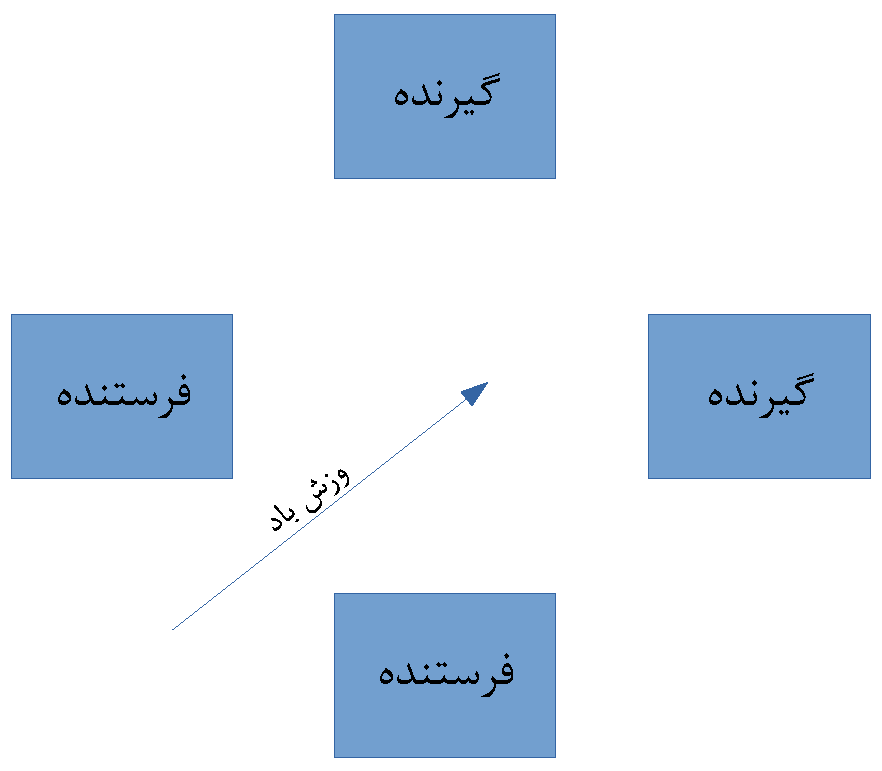
\includegraphics[width=\linewidth]{Assets/ultrasonic 2d.pdf}
		\caption{}
		\label{fig:2dUltrasonic}
	\end{subfigure}
	\begin{subfigure}[b]{0.5\textwidth}
		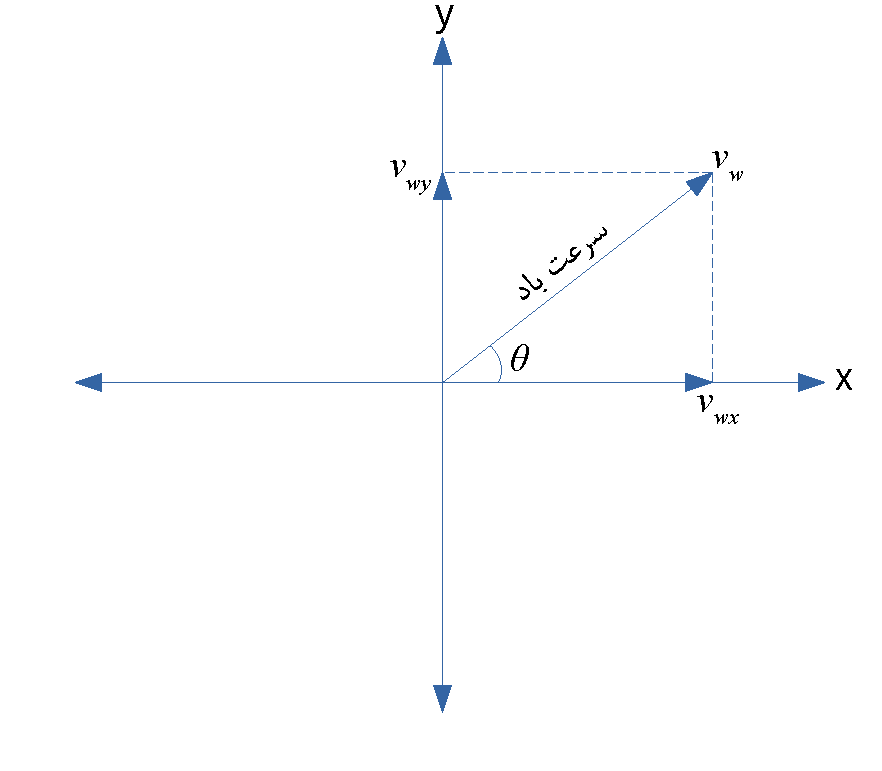
\includegraphics[width=\linewidth]{Assets/ultrasonic 2d axis.pdf}
		\caption{}
		\label{fig:2dUltrasonicAxis}
	\end{subfigure}
	\caption{نحوه قرارگیری فرستنده و گیرنده آلتراسونیک دو محوره و نمودار متناظر با آن‌ها.}
\end{figure}

اگر نحوه قرارگیری فرستنده و گیرنده‌ها مطابق شکل \رجوع{fig:2dUltrasonic} باشد در این صورت صفحه مختصات متناظر با آن مطابق شکل \رجوع{fig:2dUltrasonicAxis} خواهد بود. اندازه $v_w$ و زاویه $\theta$ بردار سرعت باد از طریق روابط \رجوع{eq:windSpeed} به‌دست می‌آیند.

\begin{equation}\label{eq:windSpeed}
	\begin{split}
		v_w = \sqrt{v_{wx}^2 + v_{wy}^2}\\
		\theta = \tan^{-1}{\left( \frac{v_{wy}}{v_{wx}}\right)}
	\end{split}	
\end{equation}

\begin{table}[!t]
	\centering
	\caption{ضرایب  محاسبه سرعت صوت (فرمول \رجوع{eq:soundSpeed}) \مرجع{cramer1993variation}.}
	\label{tb:speedOfSoundcoefficients}
	\begin{tabular}{cc}
		\hline \hline
		ضرایب & \\
		\hline
		$a_{0}$ & $331.5024$ \\
		$a_{1}$ & $0.603055$ \\
		$a_{2}$ & $-0.000528$ \\
		$a_{3}$ & $51.471935$ \\
		$a_{4}$ & $0.1495874$ \\
		$a_{5}$ & $-0.000782$ \\
		$a_{6}$ & $-1.82 \times 10^{-7}$ \\
		$a_{7}$ & $3.73 \times 10^{-8}$ \\
		$a_{8}$ & $-2.93 \times 10^{-10}$ \\
		$a_{9}$ & $-85.20931$ \\
		$a_{10}$ & $-0.228525$ \\
		$a_{11}$ & $5.91 \times 10^{-5}$ \\
		$a_{12}$ & $-2.835149$ \\
		$a_{13}$ & $-2.15 \times 10^{-13}$ \\
		$a_{14}$ & $29.179762$ \\
		$a_{15}$ & $0.000486$ \\
		\hline
	\end{tabular}
\end{table}

سرعت صوت $v_s$ به‌عنوان تابعی از دما، فشار و کسر مولی رطوبت و کربن دی‌اکسید، با استفاده از رابطه \رجوع{eq:soundSpeed} قابل‌محاسبه است \مرجع{cramer1993variation}. ثوابت$a_1$ تا $a_{15}$ در جدول \رجوع{tb:speedOfSoundcoefficients} آمده‌اند.

\begin{equation}\label{eq:soundSpeed}
	\begin{aligned}
		v_s\left(\tau, p, x_w, x_{c}\right)=& a_{0}+a_{1} \tau+a_{2} \tau^{2}+\left(a_{3}+a_{4} \tau+a_{5} \tau^{2}\right) x_{w} \\
		&+\left(a_{6}+a_{7} \tau+a_{8} \tau^{2}\right) p+\left(a_{9}+a_{10} \tau+a_{11} \tau^{2}\right) x_{c} \\
		&+a_{12} x_{w}^{2}+a_{13} p^{2}+a_{14} x_{c}^{2}+a_{15} x_w p x_c
	\end{aligned}
\end{equation}

که $\tau$ دمای هوا (برحسب درجه سلسیوس)، $p$ فشار هوا (برحسب پاسکال)، $x_w$ کسر مولی بخارآب در هوا و $x_c$ کسر مولی کربن دی‌اکسید در هوا است. $x_c$ را ثابت و برابر $400 \times 10^{-6}$ در نظر می‌گیریم. کسر مولی بخارآب در هوا $x_w$ از رابطه \رجوع{eq:x_w} به‌دست می‌آید \مرجع{rasmussen1997calculation}. 

\begin{equation}\label{eq:x_w}
	x_w=\frac{h f p_{sv}}{100 p}
\end{equation}

که $h$ درصد رطوبت هوا، $p_{sv}$ فشار اشباع بخارآب در هوا و $f$ ضریب تقویت است و از طریق روابط \رجوع{eq:f} و \رجوع{eq:p_sv} محاسبه می‌شوند \مرجع{davis1992equation}.

\begin{equation}\label{eq:f}
	f=1.00062+3.14 \times 10^{-8} p+5.6 \times 10^{-7} \tau^{2}
\end{equation}
\begin{equation}\label{eq:p_sv}
	\begin{aligned}
		p_{s v}=& \exp \left(1.2811805 \times 10^{-5} T^{2}-1.9509874 \times 10^{-2} T\right.\\
		&\left.+34.04926034-6.3536311 \times 10^{3} / T\right)
	\end{aligned}
\end{equation}

که در این روابط $T$ دمای محیط برحسب کلوین\پانویس{Kelvin} است، یعنی:
\begin{equation}
	T = \tau + 273.15
\end{equation}

\قسمت{پروتکل‌های ارتباطی}

قطعات الکترونیک نیز همانند انسان‌ها برای ارتباط با یکدیگر باید از یک زبان واحد قابل‌فهم برای هر دو طرف استفاده کنند که به این زبان‌ها پروتکل‌های ارتباطی گفته می‌شود. در این پروژه نیز همانند اکثر پروژه‌های الکترونیکی از تعدادی از این پروتکل‌ها برای برقراری ارتباط بین قطعات الکترونیکی مختلف (سنسورها، فرستنده-گیرنده‌های رادیویی و میکروکنترلر) استفاده شده است. در زیر اطلاعات کلی هر یک از پروتکل‌های ارتباطی استفاده‌شده در این پروژه آمده است.

\زیرقسمت{پروتکل \متن‌لاتین{SPI}}

این پروتکل یک رابط ارتباط سریالی سنکرون\پانویس{synchronous} (همزمان) چهار سیم است که برای ارتباط بین تنها یک \متن‌لاتین{Master} و چندین \متن‌لاتین{Slave} می‌تواند مورداستفاده قرار گیرد. خطوط ارتباطی بین \متن‌لاتین{Master} و \متن‌لاتین{Slave} شامل خط سیگنال کلاک (\متن‌لاتین{SCLK}\پانویس{Serial Clock})، خط ارسال داده از \متن‌لاتین{Master} به \متن‌لاتین{Slave} (\متن‌لاتین{MOSI}\پانویس{Master Out Slave In})، خط ارسال داده از \متن‌لاتین{Slave} به \متن‌لاتین{Master} (\متن‌لاتین{MISO}\پانویس{Master In Slave Out}) و خط انتخاب \متن‌لاتین{Slave} (\متن‌لاتین{SS}\پانویس{Slave Select} یا \متن‌لاتین{CS}\پانویس{Chip Select}). در حالت \متن‌لاتین{Full Duplex} به ازای هر \متن‌لاتین{Slave} معمولاً نیاز به یک پین انتخاب‌گر (\متن‌لاتین{SS} یا \متن‌لاتین{CS}) مجزا در سمت \متن‌لاتین{Master} خواهد بود. نحوه اتصال دستگاه‌های \متن‌لاتین{Slave}به \متن‌لاتین{Master} در شکل \رجوع{fig:SPIWiring} آمده است. 

\begin{figure}[!h]
	\centering
	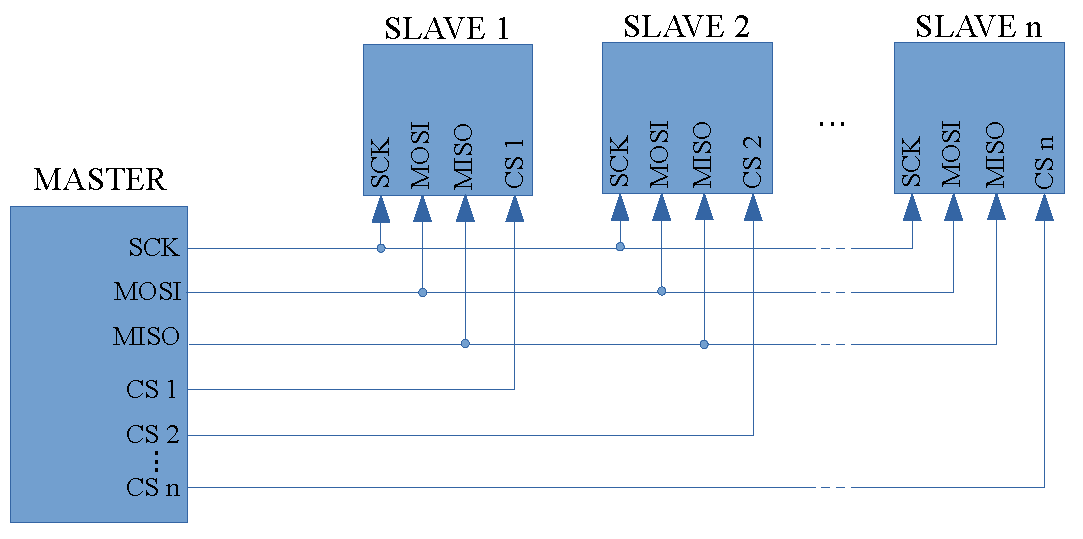
\includegraphics[width=.7\linewidth]{Assets/SPI.pdf}
	\caption{نحوه اتصال \متن‌لاتین{Slave}ها به \متن‌لاتین{Master} در حالت \متن‌لاتین{Full Duplex} }
	\label{fig:SPIWiring}
\end{figure}

سیگنال کلاک همواره توسط \متن‌لاتین{Master} تولید و به ازای هر سیگنکال کلاک یک بیت داده منتقل می‌شود. ازاین‌رو ارسال داده از \متن‌لاتین{Slave} به \متن‌لاتین{Master} به‌طور تصادفی و در هرلحظه ممکن نیست و تنها \متن‌لاتین{Slave} می‌تواند در لحظاتی که \متن‌لاتین{Master} درخواست می‌کند و سیگنال کلاک را تولید می‌کند داده را برروی خط \متن‌لاتین{MISO} ارسال کند. البته به دلیل وجود خطوط مجزای ارسال و دریافت داده، ارسال و دریافت همزمان داده نیز ممکن است. همچنین در این پروتکل دستگاه‌های \متن‌لاتین{Slave} به‌تنهایی نمی‌توانند با یکدیگر ارتباط برقرار کنند.

به جهت ارسال داده، \متن‌لاتین{Master} از طریق قراردادن خط \متن‌لاتین{SS} (یا \متن‌لاتین{CS}) در حالت \متن‌لاتین{low} انتخاب می‌کند که با کدام \متن‌لاتین{Slave} می‌خواهد ارتباط برقرار کند. وضعیت خط را تا پایان فرآیند ارسال و دریافت داده در همین حالت (\متن‌لاتین{low}) نگهمیدارد. در همین حال سیگنال کلاک را روی خط \متن‌لاتین{SCLK} متناسب با طول داده ارسالی قرار می‌دهد (ماکسیموم فرکانس کلاک بستگی به ماکسیموم مقدار قابل‌شناسایی توسط \متن‌لاتین{Slave} دارد) و داده ارسالی را نیز متناسب با کلاک روی خط \متن‌لاتین{MOSI} قرار می‌دهد (قرار دادن داده روی لبه بالارونده یا پایین‌رونده و همچنین ارسال از بیت \متن‌لاتین{MSB} یا \متن‌لاتین{LSB} بستگی به \متن‌لاتین{Slave} دارد)؛ اگر قرار باشد \متن‌لاتین{Slave} دیتایی در پاسخ به دیتای دریافتی ارسال کند (این امر باید از قبل مشخص باشد چراکه همان‌طور که گفته شد مسئول تولید کلاک فقط \متن‌لاتین{Master} است) باید \متن‌لاتین{Master} کلاک‌‌هایی متناسب با دیتای مورد انتظار برای دریافت را روی خط \متن‌لاتین{SCLK} تولید کند و دیتای مربوطه را از روی خط \متن‌لاتین{MISO} بخواند.

\زیرقسمت{پروتکل \متن‌لاتین{I\بالانویس‌متنی{2}C}}

پروتکل \متن‌لاتین{I\بالانویس‌متنی{2}C} رابط سریالی سنکرون دو سیم است که علاوه بر پشتیبانی از چندین \متن‌لاتین{Slave} قابلیت پشتیبانی از چند \متن‌لاتین{Master} را نیز دارا می‌باشد (البته \متن‌لاتین{Master}ها قادر به برقراری ارتباط با یکدیگر نیستند و از خطوط بأس به‌طور همزمان نمی‌توانند استفاده کنند). در این پروتکل برای ارتباط از تنها دو خط سیگنال کلاک (\متن‌لاتین{SCL}\پانویس{Serial Clock Line}) و سیگنال دیتا (\متن‌لاتین{SDA}\پانویس{Serial Data Line}) استفاده می‌شود. نحوه اتصال دستگاه‌ها در این پروتکل در شکل \رجوع{fig:I2CWiring} آمده است.

\begin{figure}[!h]
	\centering
	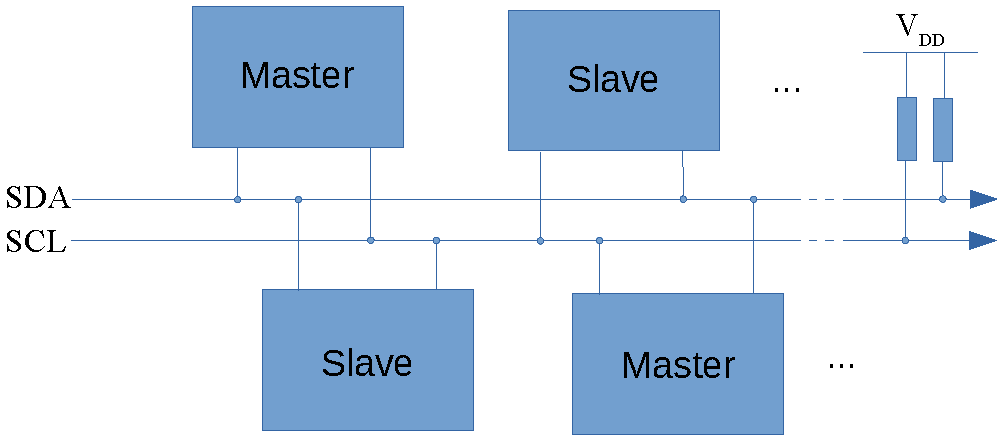
\includegraphics[width=.7\linewidth]{Assets/I2C.pdf}
	\caption{نحوه اتصال در پروتکل \متن‌لاتین{{I\بالانویس‌متنی{2}C}}}
	\label{fig:I2CWiring}
\end{figure}

در این پروتکل نیز همانند پروتکل \متن‌لاتین{SPI} سیگنال کلاک توسط \متن‌لاتین{Master} کنترل می‌شود. اعلام شروع ارسال داده با بالا نگهداشتن خط \متن‌لاتین{SCL} و پایین کشیدن خط \متن‌لاتین{SDA} انجام می‌شود. اگر دو \متن‌لاتین{Master} به‌طور همزمان قصد تبادل داده با \متن‌لاتین{Slave}ها را داشته باشند هرکدام که زودتر \متن‌لاتین{SDA} را پایین بکشید اجازه استفاده از خط را دارد و \متن‌لاتین{Master} دیگر باید تا پایان تبادلات \متن‌لاتین{Master} اول صبر کند.

برای انتقال داده پس از اعلام شروع ارسال توسط \متن‌لاتین{Master}، 7 بیت آدرس \متن‌لاتین{Slave} که قرار است با آن ارتباط برقرار شود ارسال می‌شود و پس‌ازآن یک بیت \متن‌لاتین{read/write} ارسال می‌شود تا \متن‌لاتین{Slave} از قصد \متن‌لاتین{Master} برای خواندن (سطح منطقی 1) یا نوشتن (سطح منطقی 0) مطلع شود (امکان ارتباط با \متن‌لاتین{Slave} با آدرس‌های 10 بیتی نیز وجود دارد که نحوه ارسال آن کمی متفاوت است ولی فرآیندهای دیگر در دریافت و ارسال داده‌ها یکسان است). در تمام طول ارسال و دریافت داده سیگنال کلاک نیز به‌طور منظم روی خط \متن‌لاتین{SCL} تولید می‌شود. بعد از ارسال آدرس توسط \متن‌لاتین{Master}، \متن‌لاتین{Slave}ها آدرس ارسالی را با آدرس خود مقایسه کرده و درصورتی‌که با آن مطابقت داشت بیت تصدیق (\متن‌لاتین{ACK}) را با پایین کشیدن \متن‌لاتین{SDA} تا قبل از کلاک نهم ارسال می‌کنند. اگر بیت تصدیق در این زمان ارسال نشود و \متن‌لاتین{SDA} در سطح \متن‌لاتین{high} بماند ارسال داده متوقف می‌شود چراکه عدم دریافت بیت تصدیق نشان‌دهنده عدم وجود \متن‌لاتین{Slave} موردنظر روی خط و یا عدم توانایی \متن‌لاتین{Slave} در رمزگشایی داده ارسالی است. 

پس از ارسال آدرس و دریافت تصدیق از سمت \متن‌لاتین{Slave} با توجه به بیت \متن‌لاتین{read/write} ارسالی، داده توسط \متن‌لاتین{Slave} (درحالت خواندن) و یا \متن‌لاتین{Master} (در حالت نوشتن) روی خط \متن‌لاتین{SDA} قرار داده می‌شود. بعد از ارسال هر 8 بیت داده نیز لازم است بیت تصدیق دریافت داده‌ها (\متن‌لاتین{ACK}) از طرف دریافت‌کننده داده‌ها ارسال شود. بعد از ارسال یا دریافت تمام داده‌ها باید وضعیت توقف اعلام شود تا دیگر \متن‌لاتین{Master}ها بتوانند پس‌ازآن از خط استفاده کنند. اعلام وضعیت توقف با یک تغییر وضعیت \متن‌لاتین{SDA} از سطح منطقی 0 به 1 و پس‌ازآن یک تغییر وضعیت از سطح منطقی 0 به 1  روی خط \متن‌لاتین{SCL} انجام می‌شود.

\زیرقسمت{پروتکل USB}

پروتکل \متن‌لاتین{USB} یک پروتکل ارتباطی سریال آسنکرون\پانویس{Asynchronous} (ناهمزمان) دو سیم است که ارتباطی بین چندین دستگاه جانبی یا \متن‌لاتین{Device} و دستگاه اصلی یا \متن‌لاتین{Host} را فراهم می‌کند. \متن‌لاتین{USB} توسط یک گروه متشکل از شرکت‌های فعال در زمینه رایانه و الکترونیک ایجاد شد که هدف ساخت پروتکل سریال همه‌منظوره برای اتصال لوازم جانبی به رایانه را داشتند. به دلیل همه‌منظوره بودن \متن‌لاتین{USB} استفاده از این پروتکل دارای جزئیات بسیار زیادی است و برخلاف دو پروتکل قبلی راه‌اندازی این پروتکل ممکن است زمان‌بر باشد. در این پروژه از این پروتکل برای ارتباط دستگاه سمت ایستگاه با رایانه و همچنین تأمین تغذیه آن استفاده می‌شود. نحوه اتصال دستگاه‌ها به \متن‌لاتین{Host} در شکل \رجوع{fig:USBConnection} آمده است.

\begin{figure}[!h]
	\centering
	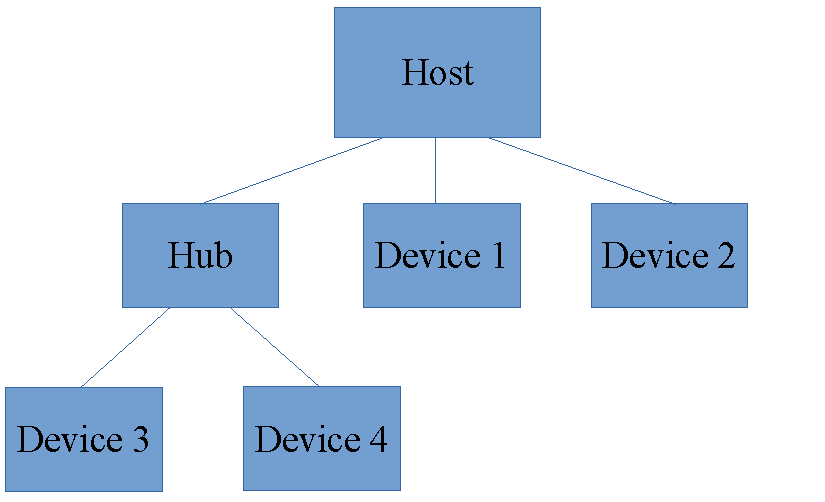
\includegraphics[width=.7\linewidth]{Assets/USB.pdf}
	\caption{نحوه اتصال دستگاه‌های جانبی به دستگاه اصلی در پروتکل \متن‌لاتین{USB}}
	\label{fig:USBConnection}
\end{figure}

به‌طورکلی برای ارتباط دستگاه‌های جانبی با دستگاه اصلی، دستگاه جانبی نیازمند دارا بودن \متن‌لاتین{Device Class} مشخص و شناخته‌شده برای دستگاه اصلی است. پیاده‌سازی دیوایس کلاس‌های اختصاصی به خاطر پیچیدگی‌هایی که این پروتکل دارد امری بسیار زمان‌بر خواهد بود به همین دلیل معمولاً استفاده از دیوایس کلاس‌های آماده (و لایبرری‌های متناطر با آن) برای ساخت دستگاه‌های جدید مناسب‌ترین روش ممکن است (این کار همچنین امر دریافت گواهی‌های سخت‌افزاری و نرم‌افزاری \متن‌لاتین{USB} را نیز تسهیل می‌کند).

در این پروتکل 4 نوع انتقال داده وجود دارد. انتقال \متن‌لاتین{Control} که تنطیمات و مشخصات دستگاه و دستورات را منتقل می‌کند. انتقال \متن‌لاتین{Isochronous} که برای انتقال داده‌هایی که زمان‌بندی در آنها اهمیت دارد نظیر صدای میکروفون و تصویر وب‌کم مورداستفاده قرار می‌گیرد. انتقال \متن‌لاتین{Bulk} که برای ارسال داده‌های حجیم‌تر به‌صورت یکجا مورداستفاده قرار می‌گیرد مانند انتقال تصویر برای پرینت و یا اسکن و یا انتقال داده‌های ذخیره‌شده روی یک فلش مموری. انتقال \متن‌لاتین{Interrupt} که داده‌هایی با حجم بسیارکم و اهمیت زیاد را جابجا می‌کند که معمولاً توسط موس، کیبرد و جواستیک (\متن‌لاتین{Joystick}) و عموماً در کلاس \متن‌لاتین{HID}\پانویس{Human interface device} مورداستفاده قرار می‌گیرد.

در این پروتکل لازم است دستگاه اصلی از تمامی جزئیات کارکرد و مشخصات دستگاه جانبی مطلع شود. مشخصات کلی دستگاه مثل ورژن \متن‌لاتین{USB} مورداستفاده، شناسه ونام سازنده، شناسه ونام دستگاه و مشخصات کلاس دستگاه در بخشی با عنوان \متن‌لاتین{Device Descriptor} با فرمتی خاص و مشخص به اطلاع رایانه می‌رسد. بخش دیگری با عنوان \متن‌لاتین{Configuration Descriptors} بیان‌کننده نحوه تغذیه و ماکسیموم توان موردنیاز دستگاه متصل به \متن‌لاتین{USB} است. بخش \متن‌لاتین{Interface Descriptors} نیز بیان‌کننده ویژگی‌های کلاس دستگاه است و شامل چندین \متن‌لاتین{Endpoint Descriptors} می‌شود که برای انجام آن ویژگی‌ها موردنیاز هستند. برای هر \متن‌لاتین{Endpoint} در سمت دستگاه جانبی ازنظر سخت‌افزاری معمولاً یک رجیستر یا مموری تعریف می‌شود که دیتا با توجه به مشخصات هر \متن‌لاتین{Endpoint} از آن خوانده می‌شود یا در آن نوشته می‌شود هر \متن‌لاتین{Endpoint} فقط مسئول یکی از اعمال خوانده شدن یا نوشته شدن است و برای هر دو عمل خواندن و نوشتن به دو \متن‌لاتین{Endpoint} نیاز است. ماکسیموم می‌توان 16 \متن‌لاتین{Endpoint} تعریف کرد، \متن‌لاتین{Endpoint} صفر رزرو و برای مشخصات کنترلی استفاده می‌شود دیگر \متن‌لاتین{Endpoint}‌ها را می‌توان با مشخات موردنیاز تعریف کرد. 

به‌طور مثال در این پروژه از کلاس \متن‌لاتین{CDC}\پانویس{Communications Device Class} استفاده‌شده است (که در کارت‌های شبکه و مودم‌ها نیز مورداستفاده قرارمی‌گیرد). برای تبادل داده با رایانه در این کلاس از ارسال نوع \متن‌لاتین{Bulk} استفاده می‌شود. پس اینترفیسی از نوع \متن‌لاتین{CDC} باید یک \متن‌لاتین{Endpoint} با دیتاتایپ \متن‌لاتین{Bulk} به‌عنوان ورودی و یک \متن‌لاتین{Endpoint} دیگر با دیتاتایپ \متن‌لاتین{Bulk} به‌عنوان خروجی داشته باشد. آدرس \متن‌لاتین{Endpoint} ورودی \متن‌لاتین{0x01} و \متن‌لاتین{Endpoint} خروجی \متن‌لاتین{0x81} تنظیم‌شده‌اند. همچنین چون قصد استفاده از \متن‌لاتین{USB} در حالت \متن‌لاتین{Full Speed} راداریم ماکسیموم سایز بسته ارسالی نیز 64 بایت تنظیم شده است. 

\قسمت{پیاده‌سازی سیستم}

عملکرد کلی سیستم جمع‌آوری داده‌ها در سمت سنسور، ارسال اطلاعات از طریق لورا به سمت ایستگاه و نمایش اطلاعات دریافت شده در سمت ایستگاه برروی رایانه است. به‌طورکلی این سیستم به دو بخش سنسور و ایستگاه تقسیم می‌شود که بخش ایستگاه خود به دو بخش دستگاه گیرنده و برنامه دسکتاپ (\متن‌لاتین{Desktop}) قابل‌تقسیم است. در سمت سنسور اجرای فرآیندها به طریق زیر است:
\شروع{فقرات}
\فقره
بعد از روشن شدن دستگاه و فعالسازی بخش‌های موردنیاز (\متن‌لاتین{peripherals})، میکروکنترلر از طریق \متن‌لاتین{I\بالانویس‌متنی{2}C} با سنسور \متن‌لاتین{BMP180} ارتباط برقرار می‌کند و ضرایب کالیبراسیو را از سنسور \متن‌لاتین{BMP180} می‌خواند این ضرایب برای محاسبه دما و فشار مورداستفاده قرار می‌گیرند \مرجع{sensortec2015digital}.
\فقره
میکروکنترلر با برقراری ارتباط از طریق \متن‌لاتین{I\بالانویس‌متنی{2}C} با سنسور \متن‌لاتین{MAX44009} مقدار رجیستر تنظیمات این سنسور را \متن‌لاتین{0x00} تنظیم می‌کند. در این حالت سنسور در پایین‌ترین سطح مصرف توان خوده قرار می‌گیرد و هر 800 میلی‌ثانیه یکبار میزان شدت نور را اندازه‌گیری می‌کند \مرجع{MAX44009}.
\فقره
با برقراری ارتباطی از طریق \متن‌لاتین{I\بالانویس‌متنی{2}C} با سنسور \متن‌لاتین{HMC5883L} و تنظیم رجیستر تنظیمات، سنسور در حالت آماده‌به‌کار و نرخ نمونه‌برداری 50 هرتز قرار می‌گیرد \مرجع{HMC5883L}.
\فقره
رجیسترهای تنظیمات ماژول \متن‌لاتین{LoRa} با برقراری ارتباط از طریق \متن‌لاتین{SPI} تنظیم‌شده و این ماژول در حالت آماده‌به‌کار قرار می‌گیرد. فرکانس این ماژول روی 433 مگاهرتز، توان آن روی 20 \متن‌لاتین{dBm}، ضریب بخش آن روی 10 و پهنای باند آن روی 31٫2 کیلوهرتز تنظیم می‌گردد (به‌منظور دریافت اطلاعات ارسالی در سمت ایستگاه نیز دقیقاً همین تنظیمات فرکانس، پهنای باند و ضریب پخش باید اعمال شوند) \مرجع{SX1278}.
\فقره
برنامه وارد حلقه اصلی کار خود شده و دما و فشار را با استفاده از سنسور \متن‌لاتین{BMP180} اندازه‌گیری می‌کند. 
\فقره
پس از اندازه‌گیری شدت نور با استفاده از سنسور \متن‌لاتین{MAX44009} \مرجع{MAX44009} و اندازه‌گیری رطوبت هوا به‌وسیله سنسور \متن‌لاتین{AHT10} \مرجع{AHT10}، جهت جغرافیایی توسط سنسور \متن‌لاتین{QMC5883L} \مرجع{HMC5883L} به‌دست می‌آید. 
\فقره
سرعت باد روی دو محور \متن‌لاتین{x} و \متن‌لاتین{y} با استفاده از سنسور \متن‌لاتین{HCSR05} و با توجه به رابطه‌ی \رجوع{eq:speedWindX} محاسبه می‌شود. سپس زاویه و شدت باد با توجه به‌سرعت باد روی هر دو محور با توجه به رابطه \رجوع{eq:windSpeed} به‌دست می‌آید.
\فقره
اطلاعات جمع‌آوری و محاسبه‌شده از طریق ماژول لورا برای گیرنده سمت ایستگاه ارسال می‌شود.
\فقره 
میکروکنترلر و سنسورها در حالت توقف\پانویس{Stop} قرار داده می‌شوند و پس از سه ساعت با رخ‌دادن آلارم\پانویس{Alarm} میکروکنترلر از حالت توقف خارج شده و فرآیند دریافت و ارسال داده‌ها را تکرار می‌کند.
\فقره 
پس از هر بار خارج شدن از حالت توقف، آلارم بعدی برای سه ساعت بعد تنظیم می‌شود.
\پایان{فقرات}

در سمت ایستگاه نیز فرآیند زیر اجرا می‌شود:

\شروع{فقرات}
\فقره 
با اتصال دستگاه از طریق کابل \متن‌لاتین{USB} به رایانه میکروکنترلر پس از فعال‌سازی بخش‌های موردنیاز، از طریق \متن‌لاتین{SPI} با ماژول لورا ارتباط برقرار کرده و رجیسترهای تنظیمات را با اطلاعات مشابه با سمت سنسور پر می‌کند و ماٰژول لورا را در حالت دریافت اطلاعات بدون توقف \پانویس{Continuously} قرارمی‌هد \مرجع{SX1278}.
\فقره 
میکرو به حلقه اصلی کار خود واردشده و پس از چک کردن وجود دیتای دریافتی در ماژول لورا، در صورت عدم وجود دیتا به حالت خواب \پانویس{Sleep} رفته و تا زمان دریافت دیتا در همان حالت باقی می‌ماند.
\فقره 
با دریافت دیتا توسط ماژول لورا وقفه‌ای خارجی رخ‌داده و میکرو را از حالت خواب بیدار می‌کند.
\فقره
میکرو کنترلر با برقراری ارتباط از طریق \متن‌لاتین{SPI} با ماژول لورا دیتای دریافت شده را خوانده و پس از بررسی یکسان بودن شناسه دریافت‌کننده با شناسه خود آن را از طریق \متن‌لاتین{USB} به رایانه ارسال می‌کند.
\فقره 
در صورت عدم وجود دیتاهای دیگر، میکرو کنترلر به حالت خواب رفته و تا رخ دادن وقفه بعدی، که نشان‌دهنده دریافت اطلاعات توسط ماژول لورا است، در همان حال باقی می‌ماند.
\پایان{فقرات}

برنامه دسکتاپ که با زبان \متن‌لاتین{Python} نوشته شده است، متشکل از سه بخش \متن‌لاتین{Home}، \متن‌لاتین{Charts} و \متن‌لاتین{Log} می‌باشد. در بخش \متن‌لاتین{Home} اطلاعات آخرین دیتای دریافت شده به نمایش درمی‌آید. در بخش \متن‌لاتین{Charts} نمودارهای دیتاهای دریافتی در بازه قابل‌تعیین توسط کاربر به نمایش درمی‌آید. تمام رخدادهایی که در ارتباط با دستگاه رخ می‌دهد نظیر دریافت دیتای جدید و یا اتصال یا قطع اتصال دستگاه در تب \متن‌لاتین{Log} با ذکر زمان لیست می‌شوند. نحوه عملکرد برنامه دسکتاپ به شرح زیر است:

\شروع{فقرات}
\فقره
با اجرای برنامه \متن‌لاتین{Thread} اصلی وظیفه ترسیم رابط گرافیکی برنامه\پانویس{Graphical user interface (GUI)}، که با \متن‌لاتین{PyQt5} پیاده‌سازی شده است، را برعهده می‌گیرد.
\فقره 
در همین حین \متن‌لاتین{Thread} دیگر به کمک کتابخانه \متن‌لاتین{libusb} مسئول بررسی وضعیت اتصال دستگاه به رایانه و دریافت اطلاعات ارسالی از دستگاه می‌شود.
\فقره 
در صورت تغییر وضعیت اتصال و یا دریافت اطلاعات، مشخصات آن در تب \متن‌لاتین{Log} ثبت می‌شود و برای کاربر قابل‌مشاهده خواهد بود.
\فقره
هنگام دریافت اطلاعات جدید از طریق \متن‌لاتین{USB} علاوه بر نمایش در تب اصلی برنامه، به‌روزرسانی تب \متن‌لاتین{Charts} با اطلاعات جدید و ثبت رخ داد در تب \متن‌لاتین{Log}، مشخصات کامل آن در دیتابیس \متن‌لاتین{SQLite} در کنار فایل اجرایی برنامه نیز ذخیره می‌شود. 
\فقره 
در تب \متن‌لاتین{Charts} با انتخاب بازه زمانی، نمودارها باتوجه به اطلاعات ثبت‌شده آن بازه زمانی در دیتابیس بروز می‌شوند.
\پایان{فقرات}

\قسمت{طراحی بردمدارچاپی}

\begin{figure}[!h]
	\begin{subfigure}[b]{0.5\textwidth}
		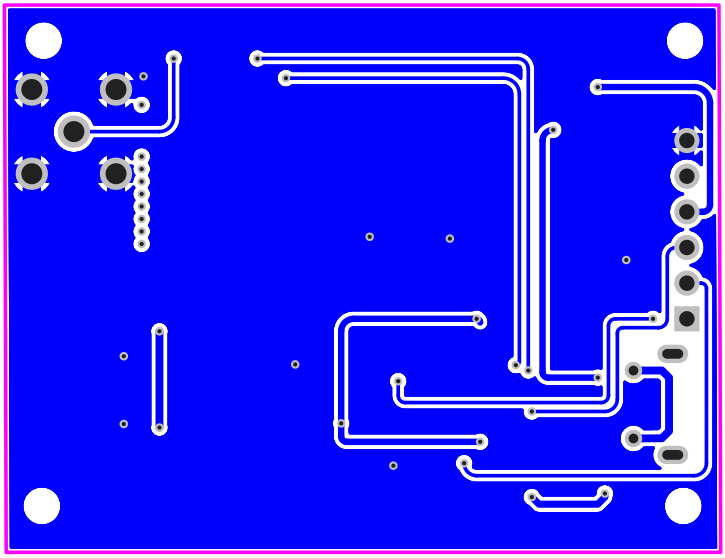
\includegraphics[width=\linewidth]{Assets/receiverBack.png}
		\caption{پشت برد سمت ایستگاه}
		\label{fig:receiverBack}
	\end{subfigure}
	\begin{subfigure}[b]{0.5\textwidth}
		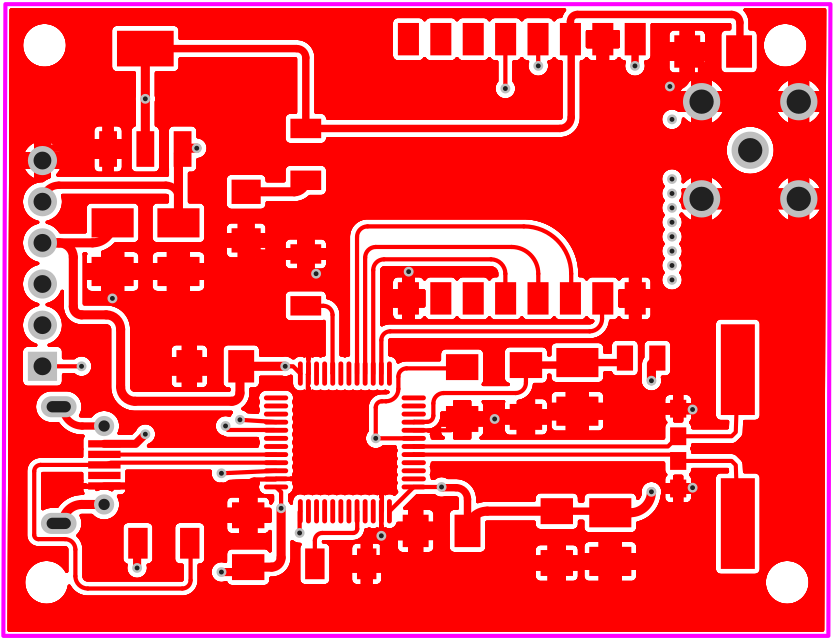
\includegraphics[width=\linewidth]{Assets/receiverFront.png}
		\caption{روی برد سمت ایستگاه}
		\label{fig:receiverFront}
	\end{subfigure}
	\begin{subfigure}[b]{0.5\textwidth}
		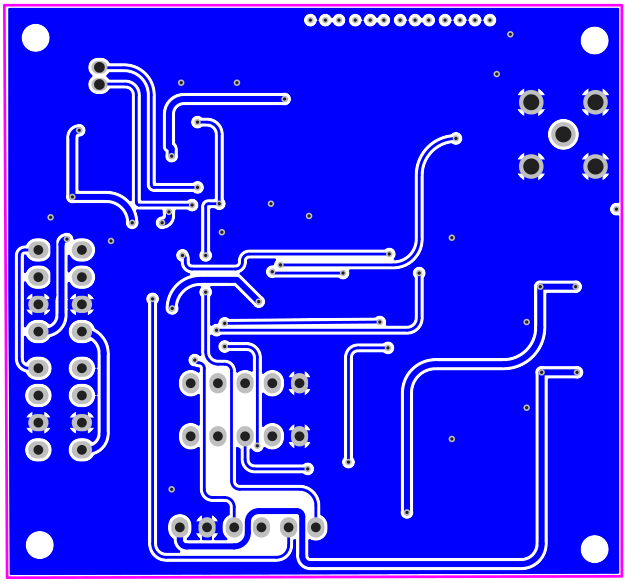
\includegraphics[width=\linewidth]{Assets/transmitterBack.png}
		\caption{پشت برد سمت سنسور}
		\label{fig:transmitterBack}
	\end{subfigure}
	\begin{subfigure}[b]{0.5\textwidth}
		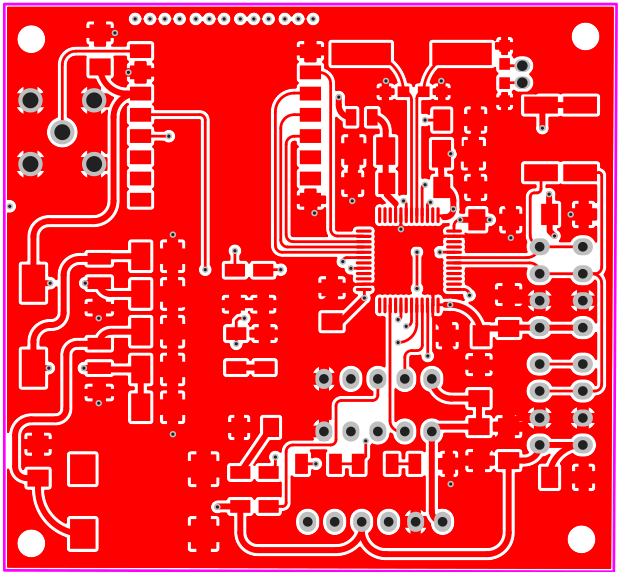
\includegraphics[width=\linewidth]{Assets/transmitterFront.png}
		\caption{روی برد سمت سنسور}
		\label{fig:transmitterFront}
	\end{subfigure}
	\caption{تصاویر بردمدارچاپی طراحی‌شده برای هر دو سمت ایستگاه و سنسور.}
	\label{fig:PCB}
\end{figure}

بردمدارچاپی\پانویس{Printed Circuit Board (PCB)} بردی است که با کانکتور و ترک‌هایی که روی آن قرار دارد قطعات را به‌طور الکتریکی به یکدیگر متصل می‌کند. بردمدارچاپی به‌طورکلی متشکل از هسته‌ای محکم معمولاً از جنس فیبرشیشه \متن‌لاتین{FR4} و لایه‌های مسی نازک که در یک یا دو طرف آن قرار دارند می‌شود. ترک‌ها و پدها روی لایه‌های مسی و پس از حل کردن مس سایر بخش‌ها در اسید به وجود می‌آیند. برای محافظت از تماس ناخواسته ترک‌های مسی با قطعات و ذرات رسانا و همچنین جدا نمودن محل‌های لحیم‌کاری از سایر بخش‌ها، بر روی لایه مسی لایه‌ی \متن‌لاتین{Solder mask} قرار می‌گیرد که معمولاً به رنگ سبز است.

یکی از موارد مهم در مرحله طراحی‌بردمدارچاپی توجه به تأثیرات نویز در مدار و تلاش به کاهش اثرات آن است. نویزها می‌تواند به دو صورت الکتریکی (در اثر خاصیت خازنی بین دو هادی) و مغناطیسی (در اثر خاصیت سلفی هادی) به وجود بیایند. منابع اصلی نویز سیگنال‌های پرودیک با فرکانس بالا نظیر زوج سیم‌های تفاضلی (\متن‌لاتین{D+} و \متن‌لاتین{D-} موجود در \متن‌لاتین{USB}) یا سیگنال‌های ساعت\پانویس{Clock} هستند. 

با عبور جریان از یک هادی میدان مغناطیسی در اطراف آن به وجود می‌آید و در صورت وجود هادی‌ای دیگر در نزدیکی آن میدان تولیدشده روی آن تأثیر گذاشته و باعث ایجاد جریان در هادی دوم می‌شود. همچنین وجود اختلاف‌پتانسیل بین دو هادی مجاور سبب ایجاد میدان الکتریکی شده و تغییرات پتانسیل یک هادی روی دیگری همانند صفحات یک خازن اثر می‌گذارد. کاهش طول هادی‌ها یکی از عوامل مؤثر در کاهش این نوع نویزها است. استفاده از خازن‌های کوپلاژ برای میکروکنترلر \مرجع{AN2586}، استفاده از فیلترهای \متن‌لاتین{RC} و \متن‌لاتین{LC}، استفاده از \متن‌لاتین{Polygon} (یا \متن‌لاتین{Pour}) و استفاده از انواع شیلد و محافظ‌های زمین شده، از روش‌ها کاهش انواع نویز هستند که در طراحی بردمدار چاپی باید به آن‌ها توجه کرد. بردهای این پروژه نیز مطابق با این نکات طراحی‌شده‌اند. تصویر بردمدارچاپی طراحی‌شده این پروژه در شکل   \رجوع{fig:PCB} آمده است.
 
\قسمت{نتایج}

\begin{figure}[!b]
	\begin{subfigure}[b]{0.5\textwidth}
		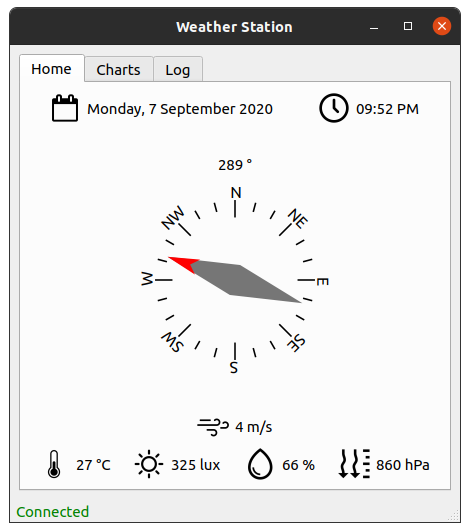
\includegraphics[width=\linewidth]{Assets/desktopAppHome.png}
		\caption{نمایش آخرین دیتاهای دریافتی برنامه در تب \متن‌لاتین{Home}.}
		\label{fig:desktopAppHome}
	\end{subfigure}
	\begin{subfigure}[b]{0.5\textwidth}
		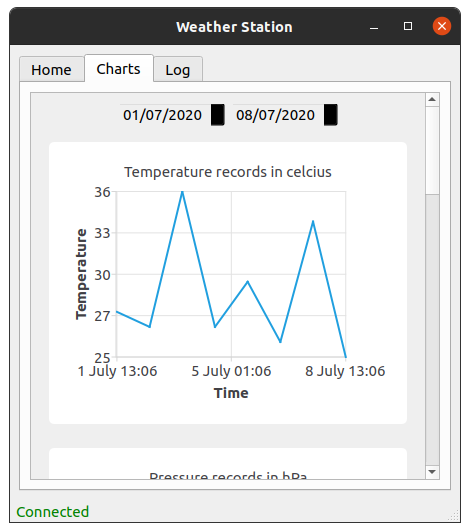
\includegraphics[width=\linewidth]{Assets/desktopAppCharts.png}
		\caption{نمایش نمودارهای اطلاعات دریافت شده در تب \متن‌لاتین{Charts}.}
		\label{fig:desktopAppCharts}
	\end{subfigure}
	\caption{تصاویر محیط برنامه دسکتاپ.}
	\label{fig:desktopApp}
\end{figure}

خروجی اطلاعات جمع‌آوری و مخابره شده توسط دستگاه بر روی رایانه و به کمک برنامه ساخته‌شده به همین منظور در سمت ایستگاه قابل‌مشاهده خواهد بود. جهت انجام بررسی‌های جزئی و ابتدایی به جهت پیش‌بینی وضعیت آب‌و‌هوایی بر روی دیتاهای دریافتی، می‌توان از نمودار دیتاهای دریافتی که در تب \متن‌لاتین{Charts} برنامه قائل مشاهده است استفاده نمود. همچنین مشخصات و جزئیات آخرین دیتای دریافت شده نیز در تب \متن‌لاتین{Home} این نرم‌افزار قابل‌مشاهده است. تصاویری از محیط برنامه در  شکل \رجوع{fig:desktopApp} آمده است.

\قسمت{نتیجه‌گیری}

در انجام تست‌های عملی مشخص شد برد مفید ماژول لورا علاوه بر وابستگی‌ای که به پارامترهای پهنای‌باند، ضریب پخش و توان دارد، به‌شدت به نوع آنتن وابسته است و نیازمند توجه ویژه‌ای به مسئله تطبیق امپدانس ترک‌های آنتن خروجی در طراحی بردمدارچاپی است. به دلیل در دسترس نبودن معیار دقیقی برای سنجش سرعت باد نتیجه‌گیری در مورد دقت اندازه‌گیری سرعت باد اشتباه است اما با انجام آزمایشات متعدد دقت اندازه‌گیری جهت باد با سرعت متوسط و در دمای اتاق 4$\pm$ درجه به‌دست آمد. همچنین مشخص شد تغییر فاصله فرستنده و گیرنده‌های آلتراسونیک از یکدیگر و از زمین، عاملی مؤثر در تعیین دقت اندازه‌گیری و ماکسیموم سرعت قابل‌اندازه‌گیری است. به‌طوری‌که با نزدیک‌تر قرار دادن فرستنده و گیرنده (تا حداقل 4 سانتی‌متر) سرعت قابل‌اندازه‌گیری ماکسیموم و دقت اندازه‌گیری مینیموم می‌شود.

\vspace{1cm}
\بدون‌تورفتگی
{\درشت سورس‌کد تمامی پخش‌های پروژه به‌صورت متن‌باز در وبگاه \متن‌لاتین{GitHub} به نشانی زیر در دسترس است:}

\begin{latin}\noindent\large
	\href{https://github.com/jmdmahdi/Weather-Station}{https://github.com/jmdmahdi/Weather-Station}
\end{latin}

\vspace{0.5cm}
